\documentclass{standalone}
\usepackage[T1]{fontenc}
\usepackage[utf8]{inputenc}
\usepackage{pgf,tikz}
\usepackage{setspace}
\usepackage{pgfplots}
%\pgfplotsset{compat=1.9}


\begin{document}

\small
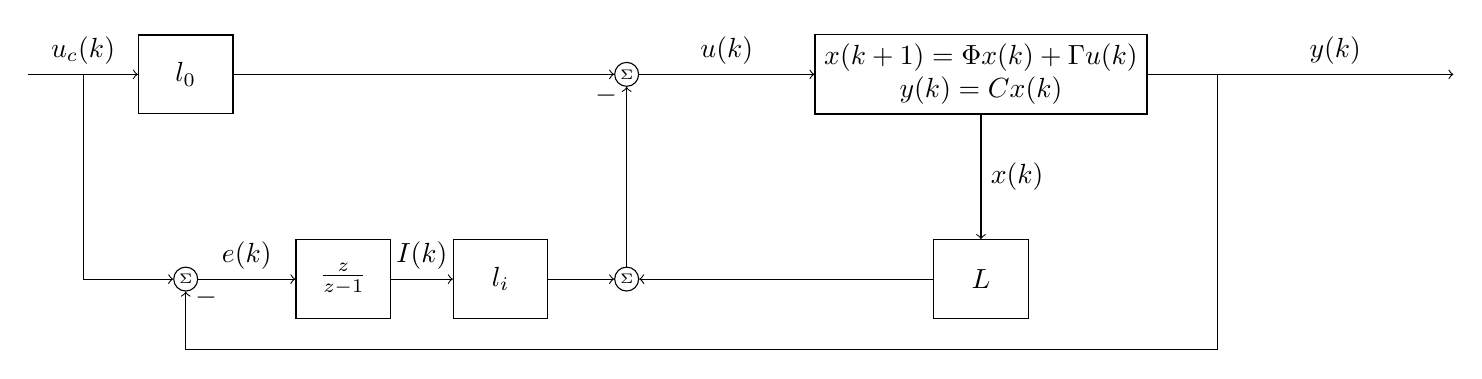
\begin{tikzpicture}[
    node distance=2cm, block/.style={rectangle, draw, minimum height=10mm, minimum width=12mm}, sumnode/.style={circle, draw, inner sep=1pt}]

    
  \node[coordinate] (input) {};
  \node[block, right of=input] (inputgain) {$l_0 $}; %l_0
  \node[sumnode, right of=inputgain, node distance=56mm] (sum) {\tiny $\Sigma$};
  \node[sumnode, below of=sum, node distance=26mm] (sum3) {\tiny $\Sigma$};
  \node[block,right of=sum, node distance=45mm, align=center] (plant) {$x(k+1) = \Phi x(k) + \Gamma u(k)$\\$y(k) = Cx(k)$};
  \node[coordinate, right of=plant, node distance=30mm] (measure) {};
  \node[coordinate, right of=measure, node distance=30mm] (output) {};
  \node[block, below of=plant, node distance=26mm] (feedbackgain) {$L$}; % L
  \node[sumnode, below of=inputgain, node distance=26mm] (sum2) {\tiny $\Sigma$};
  \node[block, right of=sum2, node distance=20mm] (int) {$\frac{z}{z-1}$};
  \node[block, right of=int, node distance=20mm] (intgain) {$l_i$};

  \draw[->] (input) -- node[above] {$u_c(k)$} node[coordinate,] (uc) {} (inputgain);
  \draw[->] (inputgain) -- node[above] {} (sum);
  \draw[->] (sum) -- node[above] (umeas) {$u(k)$} (plant);
  \draw[->] (plant) -- (measure) -- node[above] {$y(k)$} (output);
  \draw[->] (plant) -- node[right]{$x(k)$} (feedbackgain);

  \draw[->] (uc) |- node[right]{} (sum2);
  \draw[->] (measure) -- ++(0mm, -35mm) -| node[right, pos=0.95]{$-$} (sum2);
  \draw[->] (sum2) -- node[above,]{$e(k)$} (int);
  \draw[->] (int) -- node[above,]{$I(k)$} (intgain);
  \draw[->] (intgain) -- node[above,]{} (sum3);
  \draw[->] (feedbackgain) -- node[above,]{} (sum3);
  \draw[->] (sum3) -- node[left, pos=0.95]{$-$} (sum);

  
  
\end{tikzpicture}
\end{document}


